\chapter{驾驶人行为特性及对交通流影响的含义}
最基本的驾驶行为可以划分为三个不断交替的子过程,感知与信息收集,驾驶决策和对车辆的操控。感知与信息收集过程中,驾驶人主要依靠视觉采集相关的信息,这些信息来源于周围车辆和自身车辆。其中驾驶人只对部分信息变量敏感,包括速度,加速度,跟驰距离,相对速度,以及这些变量的某些函数(如时间间隔)。驾驶人收集到信息后通过采样与整合对这些信息进行解释,这种解释依靠驾驶人的对于车辆动态特性的理解以及其积累的驾驶经验。通过对信息解释的整合处理,最终形成驾驶决策。驾驶决策形成后,驾驶人通过对车辆机件的操作,对车辆的动态施加控制。而本文所研究的的驾驶人行为特性是指驾驶人通过操控车辆,使得车辆所表现出的一系列特性,而不具体研究驾驶人操控动作。其中驾驶过程框图如
\autoref{drv_blockdia}


\begin{figure}[htpb]
	\centering
	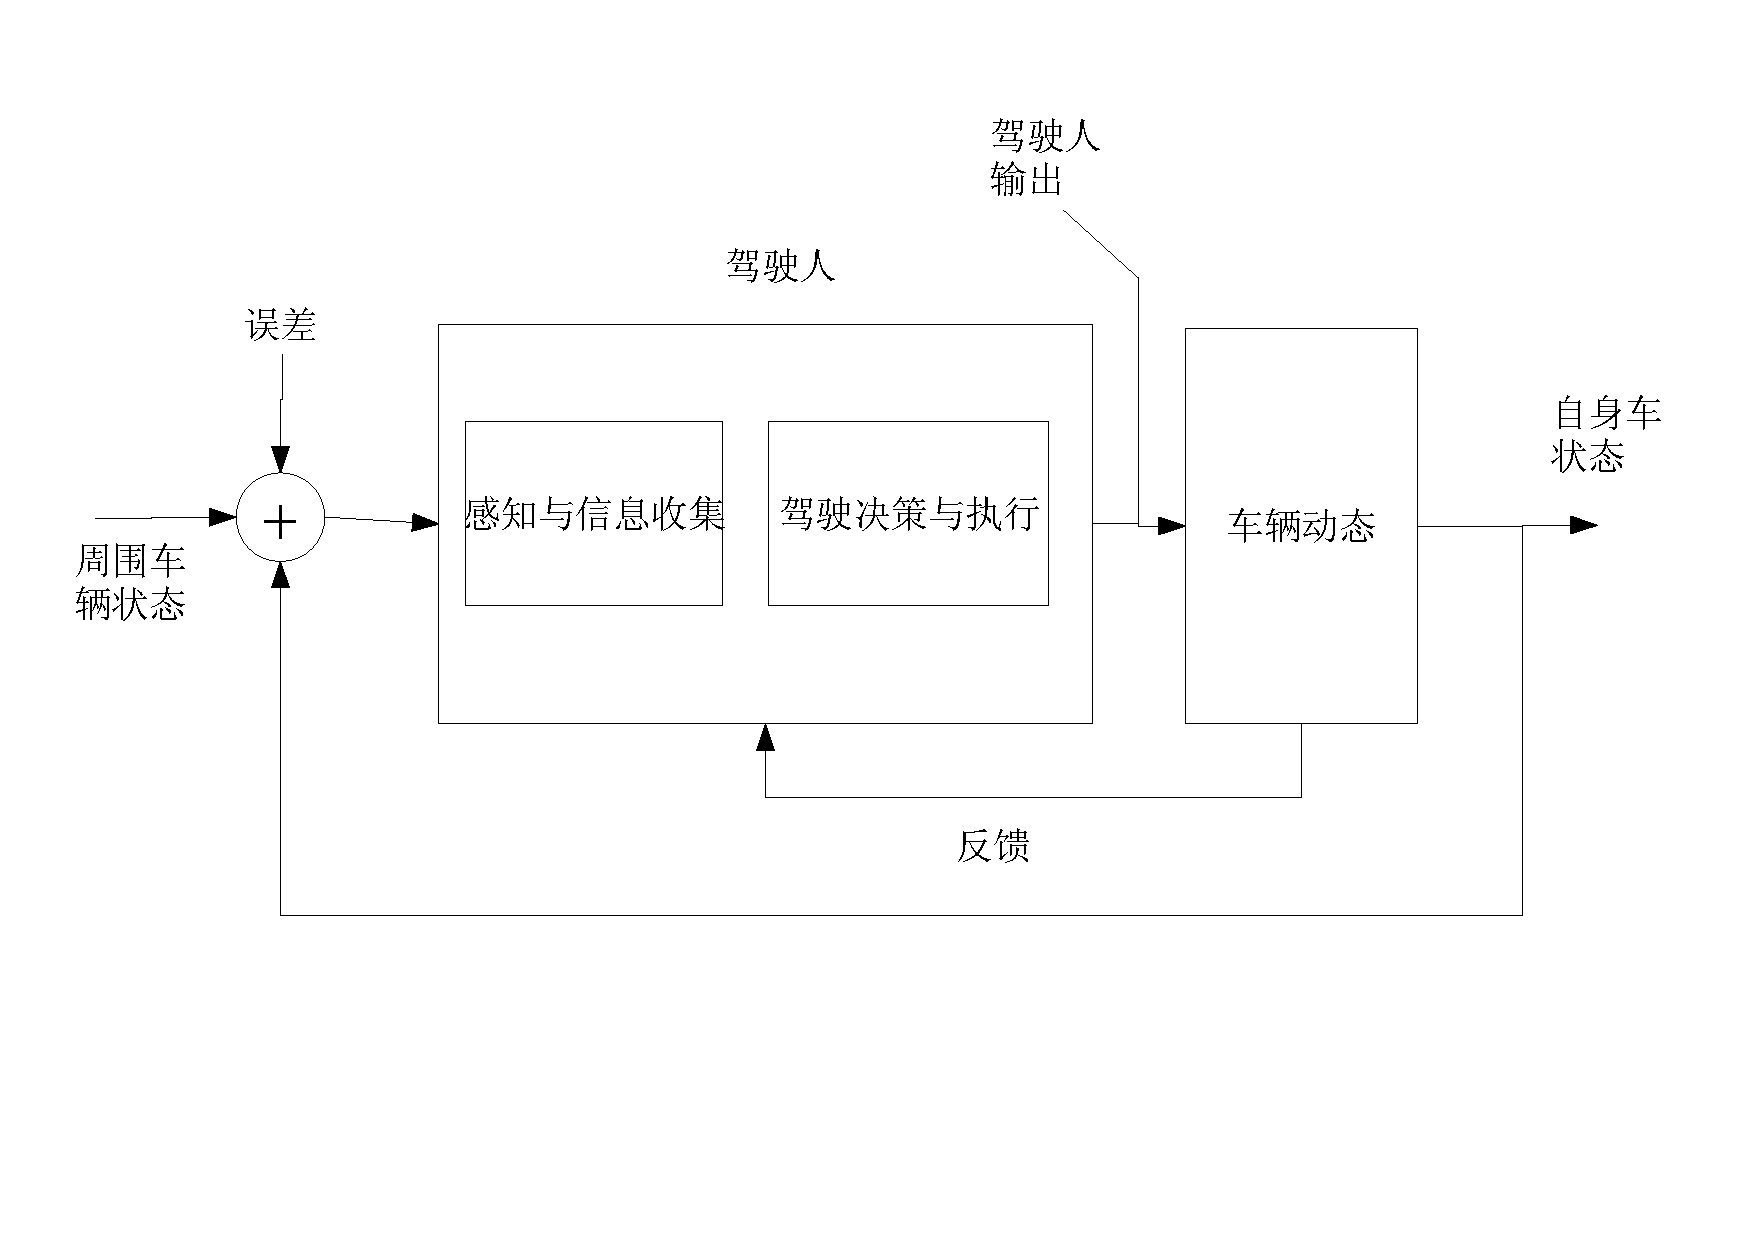
\includegraphics[totalheight=10cm]{drv_blockdia}
	\caption{驾驶过程框图}
	\label{drv_blockdia}
\end{figure}
驾驶人行为可以分为跟驰行为和变道行为,两者事实上存在紧密联系,但是现阶段主要的交通流模型研究中仍然分别对这两种行为独立地进行分析,这种两者相对独立的假设便于开展研究,并且有利于交通流模拟系统的实现。本章中将对驾驶人的跟驰和变道行为特性的内涵分别进行阐述,并分析两者的联系,最后对驾驶人行为特征影响交通流的含义进行阐述。
%\begin{table}[htbp]
% \centering
% \caption{Add caption}
% \begin{tabular}{cccc}
%   \addlinespace
%    \toprule
%    Face database & Yale  & Caltech & ORL \\
%    \midrule
%    Number of training & \multicolumn{ 1}{c}{5} & \multicolumn{ 1}{c}{3} & \multicolumn{ 1}{c}{3} \\
%    samples per class  & \multicolumn{ 1}{c}{} & \multicolumn{ 1}{c}{} & \multicolumn{ 1}{c}{} \\
%    \bottomrule
%    \end{tabular}
%  \label{tab:addlabel}
%\end{table}

\section{跟驰行为特性}

\subsection{跟驰行为特性参数}
描述微观的驾驶人跟驰行为时,对于每一个人车单元DVU(driver-vehicle-unit)(也就是外在所表现出来的车辆,下文不再对此进行区分)有若干的特性参数来反映驾驶人的行为,这些参数包括两类,一类是可以直接测量或经由简单计算所得的变量,直接测量的变量包括车辆的即时速度,即时加速度,相对速度和跟驰距离。由直接测量变量经过计算得出的变量,包括跟车对的时间间隔。第二类是不可直接或很难测得也不可经由简单计算得出的变量,这些变量也反映了驾驶人行为的重要特征,因无法直接测量,需要根据前一类变量通过估计的方法得出合理的近似值,包括驾驶人的期望速度,期望跟驰距离,反应时间,期望时间间隔。

\subsubsection{速度}
车辆速度是$v$是跟驰过程中最为基本的变量,速度为车辆单位时间内的位移,在水平面上包括沿道路轴向和横向的速度分量。在跟驰过程中,车辆的沿道路轴向速度为影响跟驰车辆对相互作用的主要因素,而在正常的跟驰过程中车辆的沿道路横向速度相对轴向很小,因此在数量上,车辆速度与车辆沿道路轴向速度几乎总是非常相近。若以道路上一点作为起点,将车辆前保险杠点的沿道路方向的位移$x$看作是时间的函数,则速度为沿道路方向的位移的一阶导数,即$v=x'$。

\subsubsection{加速度}
加速度与速度类似的包括沿道路轴向和横向的上分量,加速度是速度的一阶导数,是位移的二阶导数,即$a=v'=x''$。按照加速度可将车辆的运行状态分为三类,$a>0$时为加速状态,$a<0$时为减速状态,$a=0$时为巡航状态,驾驶人通过控制油门踏板和减速踏板的开合度改变车辆的加速度。众多的跟驰模型将加速度看作驱动人车单元状态改变的变量。

\subsubsection{相对速度}
相对速度为跟车对的速度差,为引导车辆速度值减去跟驰车辆速度值。以$v_{n-1}$表示引导车辆速度,以$v_n$表示跟驰车辆速度,则相对速度$v_r=v_{n-1}-v_n$。一般认为相对速度是跟驰过程中驾驶人接受的主要刺激,驾驶人根据前后车辆的速度差相应的调整自身车辆的行驶状态。

\subsubsection{跟驰距离与车头间距}
车头间距是跟车对车头之间的距离$s_n=x_{n-1}-x_n$。跟驰距离则指车头间距减去引导车车身的长度$l_{n-1}$,即$d_n=s_n-l_{n-1}=x_{n-1}-x_n-l_{n-1}$。跟车实验中一般容易测得的是跟车距离,一般认为当跟驰距离大于或等于最恶劣条件下的安全距离能保证不发生追尾事故,其中恶劣条件下的安全距离是指前车t时刻瞬时停止的情况下,跟驰车辆从t时刻开始从反应到制动直至完全停下所运动的距离。而跟驰模型中则更多的使用车头间距,平均的车头间距反映了交通流的密度情况。
%而最小安全距离的根据跟车对之间相对速度的关系和不同的定义而变化。

\subsubsection{时间间隔与车头时距}
车头时距为跟驰车辆车头$t$时刻在速度不变的情况下到达$t$时刻前车车头位置所需要的时间,$h_t=\frac{x_{n-1}-x_n}{v_n}$,车头时距一般通过点设备(如线圈)测量,平均车头时距反映了交通流的流量情况。时间间隔为跟驰车辆车头$t$时刻在速度不变的情况下到达$t$时刻前车后保险杠位置所需要的时间,$g_t=\frac{x_{n-1}-x_n-l_{n-1}}{v_n}$,时间间隔体现了驾驶人出于安全性考虑而保留的一定的可用于驾驶操作的余地。

\subsubsection{反应时间}
反应时间是驾驶人从外界条件发生改变的一刻开始到其控制自身车辆使其运动发生相应改变所需要的时间,此处反应时间指人车单元即车辆的总反应时间$t_l$,包括驾驶人的感知时间$t_p$,反应操作时间$t_r$和车辆机械延迟时间$t_m$,即$t_l=t_p+t_r+t_m$。


\subsubsection{期望参数}
%Gipps ?Newell模型里的期望速度?
考虑期望参数即打破了驾驶人跟驰过程是完全反应式行为的假设,期望参数考虑了驾驶人的主观愿望,也就是说驾驶人在跟驰过程中会期望达到理想的跟驰状态,并在受限制的条件下对跟驰行为进行相应的调整。理想的跟驰状态由期望参数体现,具体期望参数主要有期望速度、期望车头间距和期望时间间隔等。不同的期望参数有其特定的含义,一般意义上驾驶人所期望的跟车行驶状态要满足驾驶人对于效率性,安全性等方面的需求,下一节将对部分具体的期望参数的含义进行讨论。


%期望速度(又称为心理速度,以符号$v_{dsr}$表示)是指在特定的道路条件下,车辆行驶过程中不受或基本不受其他车辆约束的条件下其驾驶员心目中希望达到的最高“安全”速度
%
%期望速度有不同的定义(又称为心理速度,以符号$v_{dsr}$表示)是指在特定的道路和交通条件下驾驶员心目中希望达到的合宜的速度。期望速度受到诸多因素的影响,如驾驶人行程的紧迫性,驾驶习惯,同时还受到道路线行,交通流状态的约束。
%
%Mclean是第一个定义期望车速的人,他认为:“期望车速是在自由流状态下,驾驶员不受线形约束所选择的运行速度。”

%\subsubsection{期望跟驰距离}
%
%\subsubsection{期望时间间隔}

%\subsubsection{视觉扩张率}


\subsection{跟驰行为的一般模型}
\subsubsection{刺激反应模型}
刺激反应模型的基本形式为,$\text{反应}(t+\Delta t)=\text{敏感度}{\times}\text{刺激}(t)$。

刺激反应模型假设跟驰中驾驶人通过视觉感知与前车的距离以及前车后部面积在视野中的大小变化来判断与前车接近或是离去及其快慢程度,通过接受这一刺激并作出判断,实施操纵从而达到安全而紧密地跟随前车行驶。其中最为典型的刺激反应模型是Chandler等(1958),Gaziz等(1959,1961)于20世纪在美国通用汽车公司研究实验室开发的一系列模型\cite{Chandler1958,Gazis1959,Gazis1961}。

其中Gaziz等(1961)给出了最一般形式的非线性GM模型\cite{Gazis1961}。非线性GM模型基于如下假设:在时刻$t+\Delta t$跟驰车的反应依赖于跟驰车对刺激的敏感度和引导车所给的刺激强度,刺激强度以引导车与跟驰车之间的相对速度、距离的形式给出,跟驰车的反应通过加速度测得,敏感特性描绘出单位刺激的反应,$\Delta t$为反应时间。GM模型的一般形式如下式:
\begin{equation}
\ddot{x}_{n+1}(t+\Delta t)=\frac{\alpha_{l,m}[\dot{x}_{n+1}(t+\Delta t)]^m}{[x_n(t)-x_{n+1}(t)]^l}\cdot [\dot{x}_n(t)-\dot{x}_{n+1}(t)],
\end{equation}
式中:
\begin{displaymath}
{\begin{aligned}
m&-\text{对速度}\dot{x}_{n+1}(t+\Delta t)\text{的敏感性参数}\\
l&-\text{对车头间距}x_n(t)-x_{n+1}(t)\text{的敏感性参数}\\
\alpha_{l,m}&-\text{常数}\\
\end{aligned}}
\end{displaymath}



\subsubsection{期望参数模型}
%Several models were developed assuming that drivers
%try to attain some desired measure. 
期望参数模型考虑了驾驶人的主观愿望,假设驾驶人在跟驰过程中会期望达到理想的跟驰状态,理想跟驰状态的参数主要有车速,车头间距和车头时距。

Helly模型,Helly(1961)提出驾驶人的反应不仅与相对速度有关,还与期望车头间距与实际车头间距差值有关\cite{Helly1961}。其模型如下:
\begin{equation}
a_n(t)=a_1\Delta V(t-\tau_n)+a_2[\Delta x_n(t-\tau_n)-D_n(t-\tau_n)],
\end{equation}

其中$D_n$是期望车头间距,其大小受到本车速度的影响。Helly模型指出并解决了GM模型中如果两车以相同速度行驶则任何车头间距均可接受的这一缺陷。
% is the desired space headway, which depends on the subject speed.
%This model addresses a deficiency of the GM model that if two vehicles travel
%at the same speed, any value of the spacing between them is acceptable. Bekey
%et al. (1977) develop a similar model from optimal control considerations.

Koshi等(1992)提出了这一模型的非线性版本\cite{M.Koshi1992}. 
%
%Gabard et al. (1982) implement it in the SITRA-B simulation model. 

%In their model, the desired space head-
%way is given by:
他们的模型中期望车头间距给出如下:
\begin{equation}
D_n(t-\tau_n)=L_{n-1}+V_n(t-\tau_n)T,
\end{equation}
其中$L_{n-1}$为引导车长度,$T$是假定为恒定的期望车头时距。

Bando等(1995)假设驾驶人施加的加速度跟其实际车辆速度与期望速度的差值成正比,而期望速度由与前车间距决定\cite{Bando1995}。模型忽略了反应时间,其形式如下:
% assume that the acceleration drivers apply is proportional to
%the deviation of their actual speed from a desired speed, which depends on the
%leader spacing. Reaction times are ignored. The model is given by: 
\begin{equation}
a_n(t)=\alpha[DV_n(t)-V_n(t)],
\end{equation}
%where DVn
%(t) is the desired speed. The following function was proposed, but no
%behavioural or empirical justification was presented: 
其中$DV_n(t)$为期望车速,其函数给出如下,但未给出理论或实际观测的证明。

\begin{equation}
DV_n(t)=\mathrm{tan}h(\Delta X_n(t)-2)+\mathrm{tan}h(2),
\end{equation}


Addison和Low(1998)以及Low和Addison(1998)将车头间距项加入GM模型提出了新的模型\cite{Addison1998,Low1998}。
%propose a model that
%combines a desired spacing term with the traditional GM term: 
%m
\begin{equation}
a_n(t)=a_1\frac{V_n(t)^m\Delta V_n(t-\tau_n)}{\Delta X_n(t-\tau_n)^l}+a_2(\Delta X_n(t-\tau_n)-D_n(t-\tau_n))^3,
\end{equation}
其期望车头间距的形式给出如下:
\begin{equation}
D_n(t-\tau)=\lambda V_n(t-\tau),
\end{equation}

Treiber等(2000)和Treiber和Helbing(2003)假设加速度受到期望速度和期望最小车头间距的影响,其模型还考虑了车辆性能的影响,但同样忽略了反应时间\cite{Treiber2000,Treiber2003}。其形式如下:
% assume that the acceleration is
%affected by both the desired speed and the desired minimum space headway. The
%model also incorporates the impact of vehicle capabilities, but ignores reaction
%time: 
\begin{equation}
a_n(t)=a_{max}\left[1-\left(\frac{V_n(t)}{DV_n(t)}\right)^\beta-\left(\frac{D_n(t)}{\Delta X_n(t)}\right )^2\right],
\end{equation}
其中$a_{max}$为车辆的最大加速度,$\beta$为参数,其最小车头间距给出如下:
%where a
%max
% is the maximum acceleration; and β  is a parameter. The desired mini-
%mum space headway is given by: 
\begin{equation}
D_n(t)=\Delta X_{jam}+V_n(t)T_n(t)+\frac{V_n(t)\Delta V_n(t)}{2\sqrt{a_{max}a_{comf}}},
\end{equation}


\subsection{本文关注的跟驰行为特性}
本文的目的在于研究驾驶人行为特性对交通流的影响,除了研究单独的行为特性参数,将着重关注可能对交通流状态产生显著影响的跟驰行为特性。直观上,速度-跟驰距离特性对于交通流效率有较大影响,而加速度-相对速度特性对于交通流稳定性和安全性有较大影响。这两方面是驾驶人跟驰过程中最为基本的任务,速度和加速度的选择既有本质的区别又存在联系。速度的选择体现了跟驰过程中驾驶人一种相对稳定的需求(例如对于安全性和执行出行计划的需要),加速度的选择则体现了驾驶人跟驰过程中对于驾驶环境的适应以及驾驶状态的改变;而两方面的联系在于,速度-跟驰距离状态的改变需要通过驾驶人施加操作来实现,也就是说速度的改变通过加速度来实现。本文将在实际测量数据的基础上,对驾驶人一般的和个体的跟驰行为特性进行研究,以期加深对驾驶人跟驰行为特性的认识。
\subsubsection{速度-跟驰距离选择}
速度-跟驰距离选择反应了驾驶人跟驰行为特性中相对稳定的部分,一方面,驾驶人根据出行计划,道路条件,交通流条件来选择车速,当车辆的加速度小于一定的阈值时则认为处于稳定的跟驰状态,此时驾驶人根据其选择的车速会与引导车保持一定的安全跟驰距离。另一方面,由于驾驶人对于外界条件的估计存在误差以及对于自身车辆的控制存在不稳定性,车辆的行驶状态会与驾驶人期望的状态出现偏差,驾驶人需要在一定的跟驰距离下调整自身相应的车速。因此驾驶人的速度-跟驰距离选择是一种组合性的选择。对于驾驶人的速度-跟驰距离选择特性研究的最为经典的结论为Newell(1961)模型。

Newell(1961)研究了速度与车头间距的关系,其假设为车速为车头间距的非线性函数\cite{Newell1961}:
\begin{equation}
V_n(t)=G_n[\Delta X_n(t-\tau)],
\end{equation}
函数$G_n$的形式体现了驾驶人的跟驰行为,Newell(1961)研究了$G_n$的具体形式\cite{Newell1961}:
\begin{equation}
V_n(t)=V_{max}\left[1-exp\left(\frac{-\lambda}{V_{max}}(\Delta X_n(t-\tau)+D)\right)\right],
\end{equation}
其中$V_{max},\lambda$和$D$为参数。$V_{max}$和$\lambda$可以相应的理解为最高车速和最小车头间距。
跟驰距离与车头间距相差的部分为引导车的车身长度,跟驰距离与车头间距两者虽不存在固定不变的算术关系,但是两者的相关性是客观存在的。跟驰模型中出于简便的需要一般使用车头间距,而不是实际中更容易测的跟驰距离。

本文将在现有研究以及实测数据的基础上对驾驶人的速度-跟驰距离选择特性进行分析,研究其在驾驶人中的差异性,并通过模拟的方法研究其对交通流的影响。


%Spacing models.  Spacing models hypothesize that the driver reacts to the leader
%spacing rather than to the relative speed. Newell (1961) assumes that the subject’s
%speed is a non-linear function of the spacing to the leader: 
%The form of the $G_n$
% function specifies the car-following behaviour. Newell (1961)
%studies the properties of the functional form: where $V_{max}$
%, λ  and $D$ are parameters. $V_{max}$
% and $D$ can be interpreted as the maximum speed and the minimum space headway, respectively.
%The acceleration the driver applies, which can be calculated by taking the
%derivatives of both sides of the above equation, corresponds to a non-linear GM
%model, with a sensitivity function that is an exponential function of the spacing.
%Newell studies the macroscopic properties of this model, but does not attempt to
%estimate the model parameters.
%Kometani and Sasaki (1958, 1959) propose a model based on the assumption


\subsubsection{加速度-相对速度选择}
加速度-相对速度选择反应了驾驶人跟驰行为特性中相对随机的部分。按照刺激反应模型的假设,驾驶人在一定的相对速度下选择相应的合适的加速度。现有的研究中,Herman等(1958)讨论了基于刺激反应模型的交通流局部和渐进稳定性\cite{Herman1959}。结果表明驾驶人的敏感性参数与反应时间的乘积决定了单车道交通流的局部和渐进稳定性。因此驾驶人的加速度-相对速度选择特性对于交通流存在不可忽略的影响。驾驶人的加速度行为的一个重要特征是加速和减速的不对称性,Forbes(1963)发现驾驶人加速过程中的反应要比减速过程中的慢\cite{Forbes1963}。Foote(1965)跟踪观测了隧道中的车队,发现在同样车速下减速车队具有更高的流量\cite{Foote1965}。Newell(1965)解释了驾驶人加减速的不对称性,认为如果前车加速跟随车会空出一段距离再做决定\cite{Newell1965}。


本文将在现有研究以及实测数据的基础上对驾驶人的加速度-相对速度选择特性进行分析,研究其在驾驶人中的差异性,并通过模拟的方法研究其对交通流的影响。
%驾驶人的加速选择对于交通流稳定产生影响,目前的研究中考虑了交通流的局部稳定性和渐进稳定性。局部稳定性是指引导车和跟驰车两辆车在特定的速度、加速度初始条件下,驾驶人通过操作是否会发生碰撞的性质,若不会发生碰撞则局部稳定,否则为局部不稳定。而渐近稳定性是指

%关于驾驶人跟驰过程的加速度-相对速度选择特性,
%
%研究发现驾驶人的加速过程以及减速过程中存在不对称性,
%
%的研究表明驾驶人的加速度值会摆动ocsilatory
%
%加速度-相对速度选择还关系到交通流的稳定性stability
%
%所以从实测的角度分析这种选择的差异性
%memory-less?
%
%extende filed of view(multi follow)
%
%planning, anticipation
%
%not myopic state



%\subsection{跟驰行为差异性}

%\subsubsection{跟驰行为内部的差异性}
%multi regime
%Wang Hao的研究表明
%This paper presents a methodology for studying the intra-driver heterogeneity of driving behavior between the acceleration process and the deceleration process with the vehicle trajectory data. The trajectory data collected from peak hours in Dutch Motorway A2 is used in this paper. Some criteria are proposed for the selection of sub-trajectories corresponding to both the acceleration and the deceleration processes of car-following. By applying these sub-trajectories to calibrate three different types of models, namely, the Helly model, the Gipps model and the IDM model, it is found that obvious intra-driver heterogeneities exist in the driving behaviors between the acceleration and deceleration processes of car-following: (a) the average response time of drivers in acceleration process is longer than that in deceleration process according to the prediction of the Helly model and IDM model; (b) drivers are apt to respond more intensively to the surrounding traffic in deceleration process than they do in acceleration process; (c) more than 65\% of drivers involved in this study drive in obviously different styles between the acceleration and the deceleration process. Moreover, the compensation for the response delay from model parameters is observed, and all the three models present low robustness in predicting driving behaviors of one car-following process with the parameters optimized from the data of the other different car-following process. This work not only presents a deep insight into the intra-driver heterogeneity in car-following behaviors, but also suggests some important criteria for car-following modeling.


%\subsubsection{驾驶人之间跟驰行为的差异性}
%\subsubsection{不同跟车对的跟驰行为的差异性}

\section{变道行为特性}

\subsection{变道行为特性参数}
描述微观的驾驶人变道行为时,对于每一个人车单元DVU同样有若干的特性参数来反映驾驶人的行为,与跟驰行为不同的是,变道行为更多时候是驾驶人主动的行为,这也意味着描述变道行为的变量有更多的不可测量的隐藏变量。

%研究驾驶人的变道行为相比跟驰行为要复杂很多。在实际观测中,首先只能观测到驾驶人发生变道的行为,也就是最终接受了间隙的结果。其次驾驶人何时做出了换道的决定通常观测不到,并且换到是连续的过程,当驾驶人作出换道的决定后还有可能寻找其他的间隙或改变换到的决定。

\subsubsection{车道属性}
车道属性包括车道平均速度,车道平均密度,和车道车辆组成等。这些变量是基于效应的模型中驾驶人所选择车道的效用主要的解释变量。驾驶人根据根据自身的观察,一般会对其周围局部的车道属性形成一定的判断。因此车道属性只在一定的时空范围内影响驾驶人的选择车道的效用。

\subsubsection{邻车速度}
驾驶人车辆周围的车辆的速度对于驾驶人的变道行为存在影响,首先周围车辆的速度影响驾驶人的车道选择,其次在驾驶人的目标车道上的前后车车速与自身车辆的车速差影响驾驶人的最小接受间隙。

\subsubsection{间隙}
间隙是指驾驶人在变道间隙接受过程中在与其相邻的目标车道上假设其变道后,前向和后向的净间距$G_f$和$G_b$,其示意图如\autoref{gap_accpet}。当目标车道上的车辆与驾驶人车辆在沿道路方向存在重叠时,间隙可为负值。
间隙接受示意图如\autoref{gap_accpet}
\begin{figure}[htpb]
	\centering
	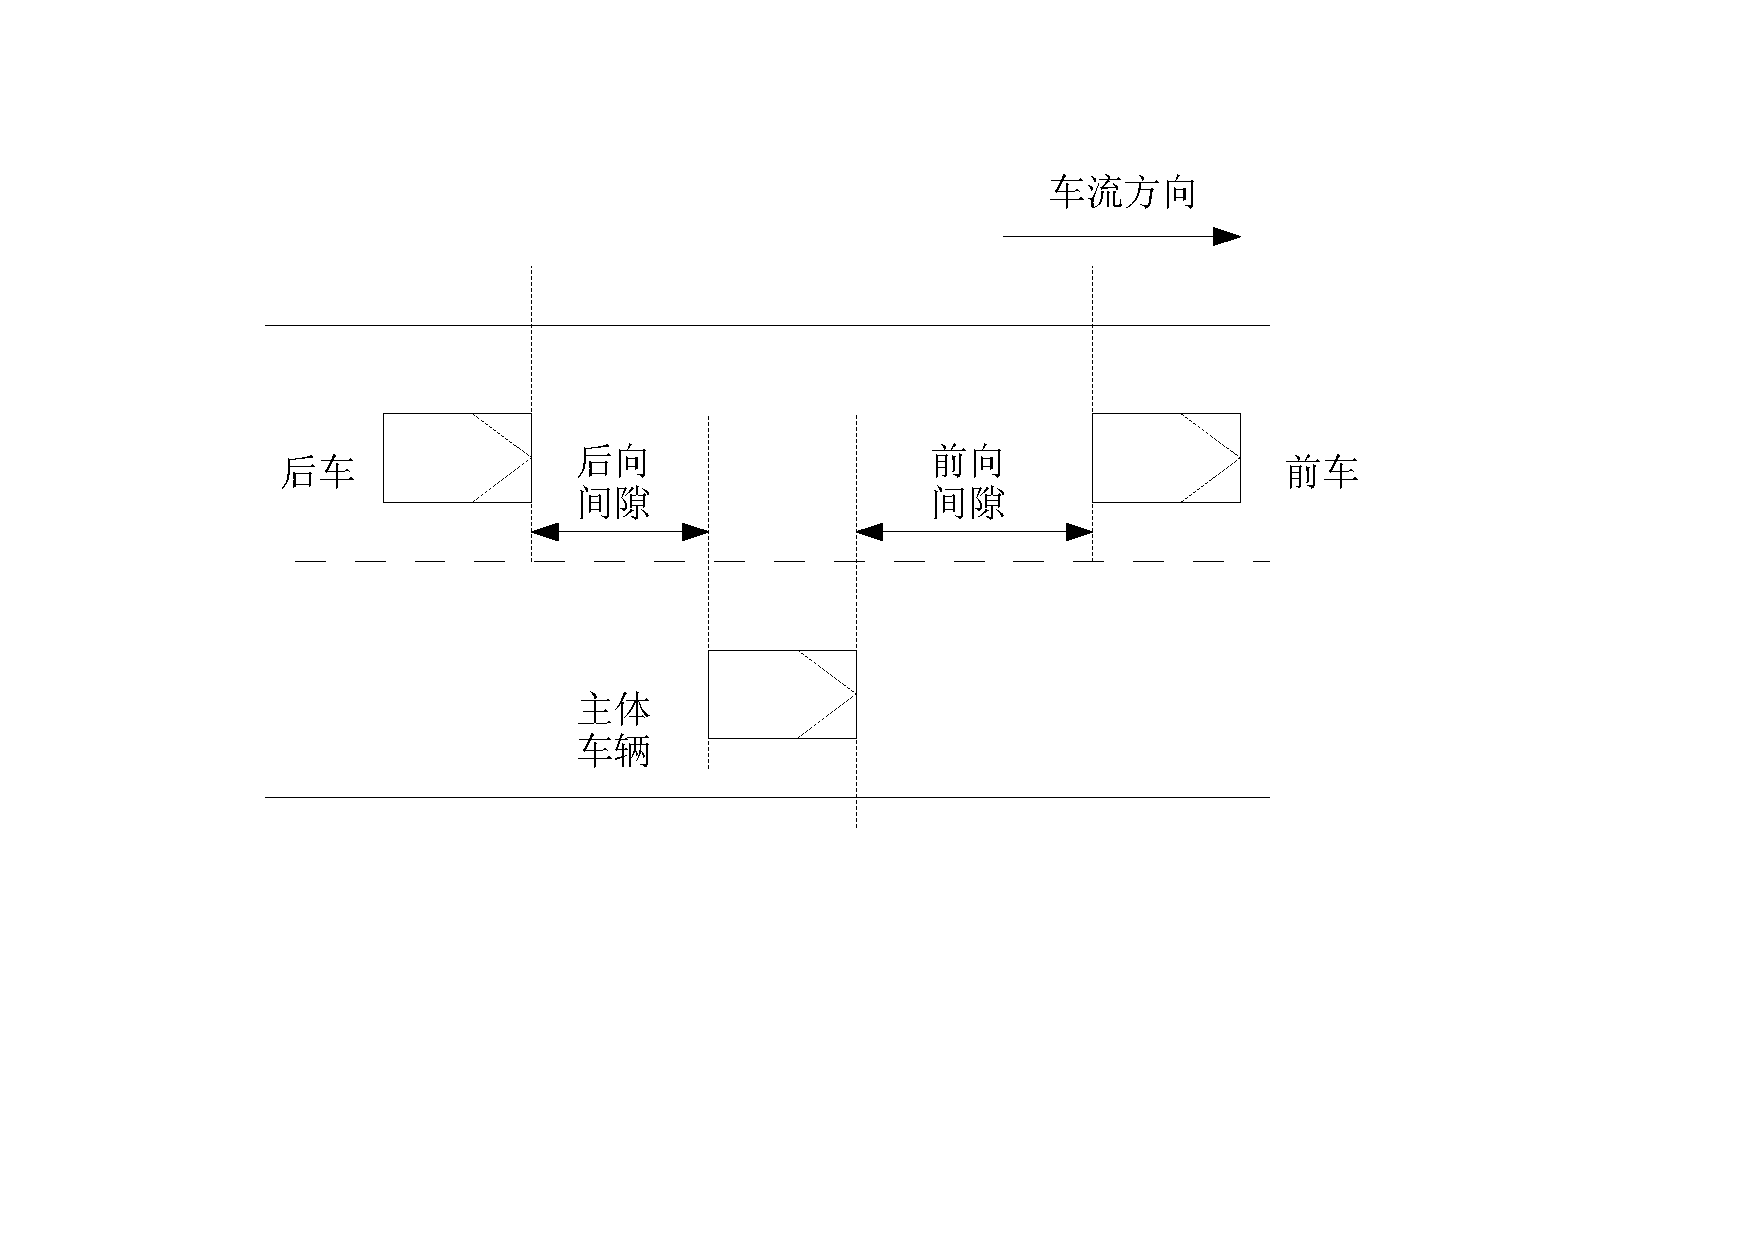
\includegraphics[totalheight=10cm]{gap_accpet}
	\caption{间隙接受示意图}
	\label{gap_accpet}
\end{figure}

\subsubsection{最小接受间隙}
最小接受间隙是指在驾驶人的间隙接受过程中,驾驶人最小的可接受间隙,当实际间隙大于最小接受间隙时则接受间隙进行变道,否则就拒绝间隙保持原车道行驶。
%目前的研究中对驾驶人的最小接受间隙分布进行了分析。

%\subsubsection{加速度改变}
%加速度改变是MOBIL模型中的驾驶人的效用函数,是指驾驶人在假设变换到目标车道以后可以获得的加速度改变(通常是增加)。
%
%\subsubsection{礼让系数}
%礼让系数

\subsection{变道行为的一般模型}
%目前描述变道行为的模型主要有两类,一类是基于车道效用和间隙接受的模型,另一类为MOBIL模型。
变道行为可分为两个阶段,第一阶段选择车道,如果选择车道非现行车道则进行第二阶段执行变道。两个阶段对应的模型分别为目标车道模型和间隙接受模型。
\subsubsection{车道选择模型}

Gipps(1986)最早提出了用于微观仿真的变道模型\cite{Gipps1986}。其模型考虑变道的必要性,可能性和安全性。驾驶人行为考虑两条最基本的原则:保持理想的速度和保持在正确的车道上从而进行计划的转向操作。

Halati等(1997)在CORSIM中提出了MLC和DLC的区别\cite{Halati1997}。按照迫切程度,变道行为可分为MLC(mandatory lane change)强制变道和DLC(discretionary lane change)选择变道,MLC强制变道指驾驶人按照行驶计划的路径必须选择某条车道时的变道行为(例如左转必须使用左转车道或下游拥堵),DLC选择变道则指驾驶人为了追求更为有利的驾驶条件而相对自由进行选择的变道行为。




 


%The first lane-changing model intended for micro-simulation tools was introduced by 
%Gipps (1986). The model considers the necessity, desirability and safety of lane-changes. 
%Drivers’ behavior is governed by two basic considerations: maintaining a desired speed 
%and being in the correct lane for an intended turning maneuver. The distance to the 
%intended turn defines which zone the driver is in and which of the considerations are 
%active. When the turn is far away it has no effect on the behavior and the driver 
%concentrates on maintaining a desired speed. In the middle zone, lane-changes will only 
%be considered to the turning lanes or lanes that are adjacent to them. Close to the turn, the 
%driver focuses on keeping the correct lane and ignores other considerations. The zones are 
%defined deterministically, ignoring variation between drivers and inconsistencies in the 
%behavior of a driver over time. When more then one lane is acceptable the conflict is 
%resolved deterministically by a priority system considering locations of obstructions, 
%presence of heavy vehicles and potential speed gain. No framework for rigor estimation 
%of the model’s parameters was proposed.  
Yang和Koutsopoulos(1996)在MITSIM中实现了一个基于规则的变道模型\cite{Yang1996}。模型中同样区分了MLC和DLC。驾驶人当需要按计划行驶至下一个连接,绕开下游的拥堵,遵守车道使用规则时进行MLC强制变道,其目标冲突通过概率的效用最大化模型解决。而当驾驶人认为引导车速度低于期望速度时考虑进行选择变道DLC,随后驾驶人寻求机会变换到相邻的车道以提高车速。其与以往模型不同之处在于车道选择基于随机的效用模型,体现了驾驶人权衡不同因素(比如速度优势,重车,汇如交通等)对车道选择的影响。
%implemented a rule based lane-changing model in 
%MITSIM where lane changes are classified as MLC and DLC. Drivers perform MLC to 
%connect to the next link on their path, bypass a downstream lane blockage, obey lane-use 
%regulations and respond to lane-use signs and variable message signs. Conflicting goals 
%are resolved probabilistically using utility maximization models. DLC are considered when the speed of the leader is below a desired speed. The driver then checks the 
%opportunity to increase speed by moving to a neighbor lane.  

Ahmed等(1996)和Ahmed(1999)提出了一个基于效用的包含MLC和DLC的通用的模型框架\cite{Ahmed1996,Ahmed1999}。变道过程分三步:决策进行变道,目标车道选择和间隙接受。当不存在MLC条件或驾驶人决定不执行MLC时,进而分两步考虑DLC。首先驾驶人检查自身车道的驾驶条件是否达到满意的程度,这取决于自身车速与期望车速的差值。如果驾驶人对自身车道的驾驶条件不满意,则驾驶人比较自身车道与相邻车道的驾驶条件,其中相邻车道的效用受到车道上的前向和后向车辆车速的影响。
 
%develop a general utility-based framework that captures both MLC and DLC situations. The lane-changing process is modelled with three steps: a decision to consider a lane change, a choiceof a target lane, and the acceptance of gaps in the target lane. If an MLC situationdoes not apply or the driver chooses not to respond to it, a decision whether to consider a DLC is made using a two-step process. First, drivers examine theirsatisfaction with driving conditions in the current lane, which is affected by the difference between the subject speed and its desired speed. The model also captures differences in the behaviour of heavy vehiclesand the effect of the presence of a tailgating vehicle. If the driving conditions in the current lane are not satisfactory, the driver evaluates conditions in neighbouring lanes and in the current lane in order to choose the target lane. The utilities of neighbouring lanes are affected by the speeds of the lead and lag vehicles in these lanes and the current and desired speed of the subject vehicle. A gap-acceptance model is also included within the lane-changing framework. 


Ben-Akiva等(2006)总结了驾驶人一般的车道选择的逻辑\cite{Ben-AkivaM.2006}。
驾驶人一般的变道逻辑图如\autoref{lc_logic}
\begin{figure}[htpb]
	\centering
	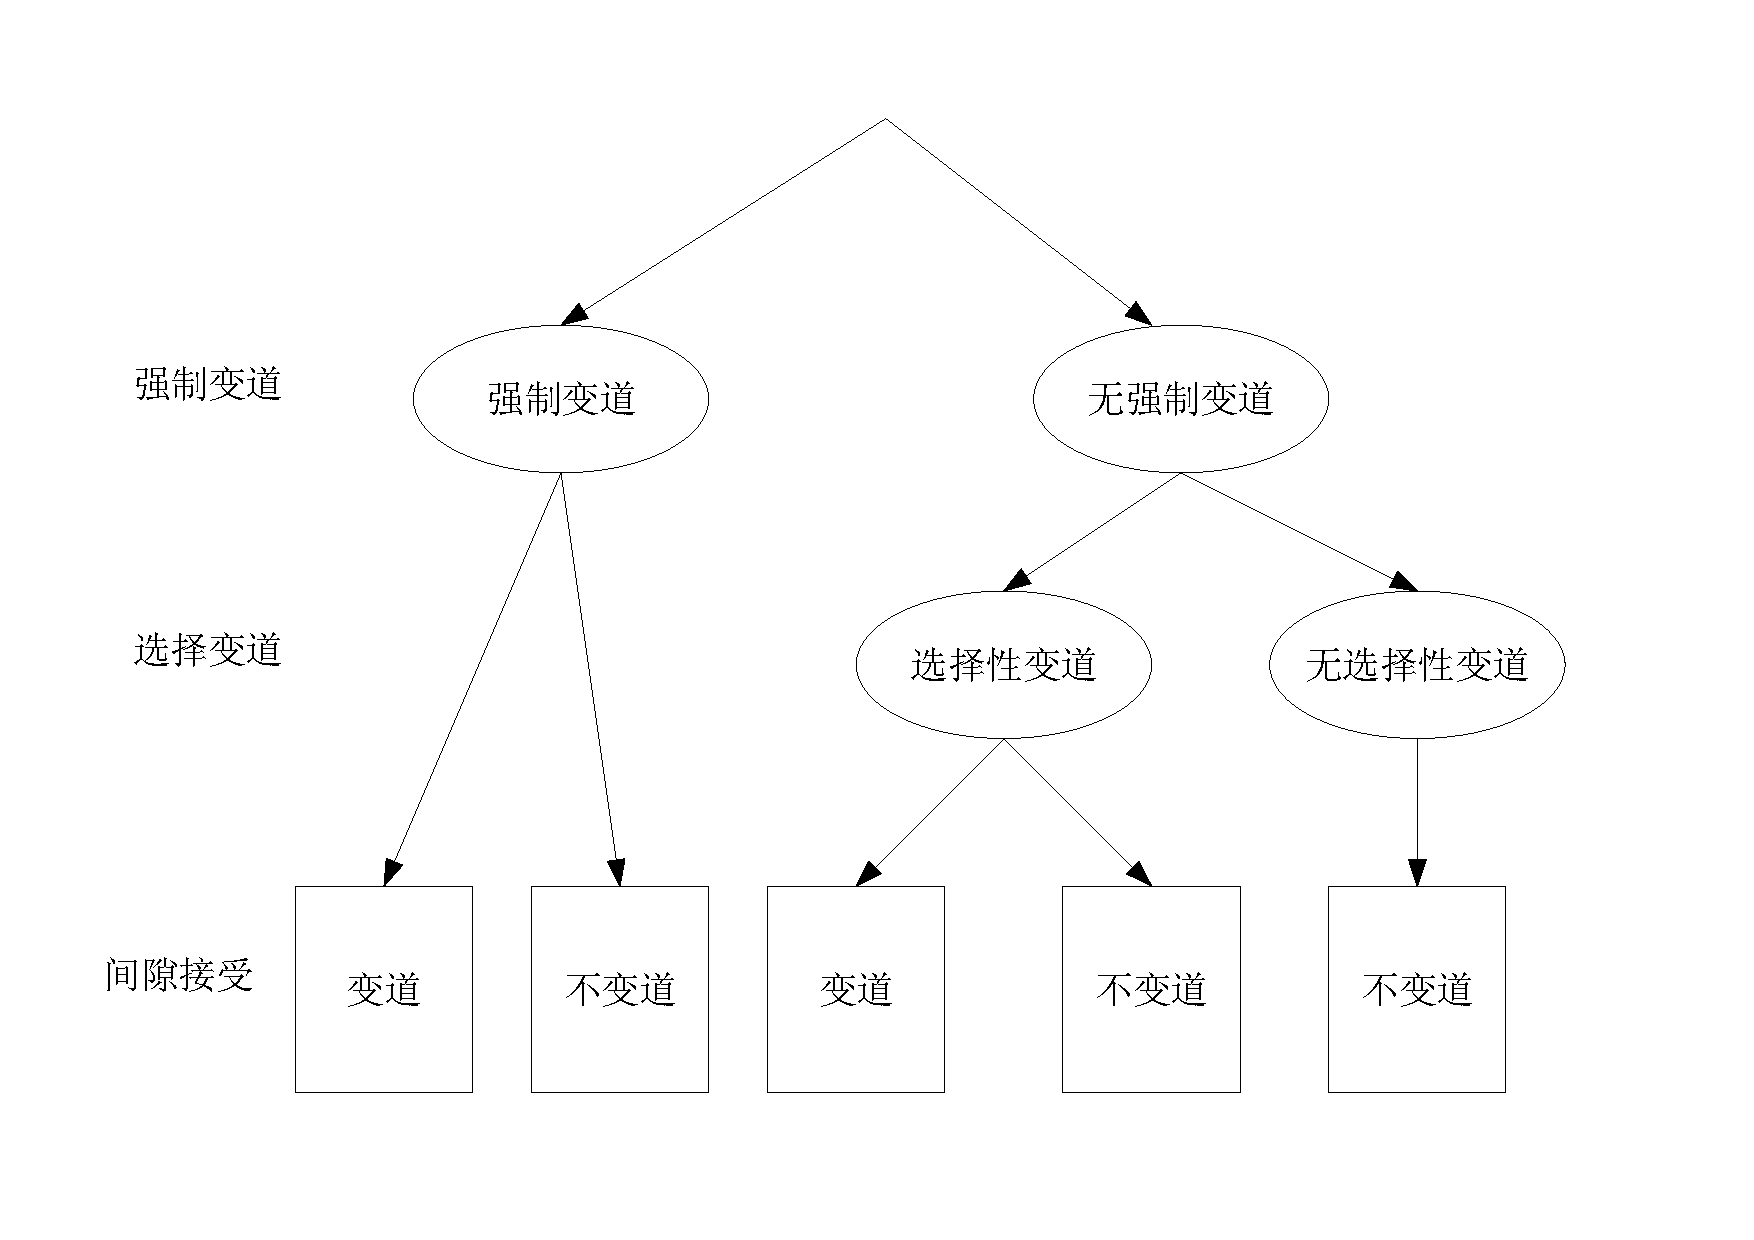
\includegraphics[totalheight=10cm]{lc_logic}
	\caption{变道逻辑图}
	\label{lc_logic}
\end{figure}


Toledo等(2005)提出了明确目标车道的车道选择模型,该模型基于效用理论并综合考虑了MLC和DLC,驾驶人选择效用最高的车道作为目标车道。目标车道的选择集包含所有驾驶人可能使用的车道,各条车道的效用函数形式如下:
\begin{flalign}
U_{int}^{TL}=\beta_{i}^{TL}X_{int}^{TL}+\alpha_{i}^{TL}v_n+e_{int}^{TL}\nonumber \\
\begin{split}
\forall i \in \mathrm{\{lane 1, lane 2, lane 3, lane 4, ...\}},
\end{split}
\end{flalign}
其中\\
\begin{displaymath}
{\begin{aligned}
U_{int}^{TL}&-\text{驾驶人}n\text{在时刻}t\text{选择车道}i\text{为目标车道的效用} \\
X_{int}^{TL}&-\text{影响车道}i\text{效用的解释变量构成的向量}\\
\beta_{i}^{TL}&-\text{与}X_{int}^{TL}\text{相对应的参数}\\
v_n&-\text{与驾驶人个体特征相关的解释变量构成的向量}\\
\alpha_{i}^{TL}&-\text{与}v_n\text{相对应的参数}\\
e_{int}^{TL}&-\text{影响驾驶人}n\text{在时刻}t\text{选择}i\text{车道效用的随机项}\\
\end{aligned}}
\end{displaymath}

模型中目标车道的效用受到车道属性(如密度,速度),以及与路径计划相关变量(如到下一个路径中指定车道的距离)的影响。除此之外,驾驶人车辆所处的车道位置也对车道选择产生影响,并在模型中通过需要变道的次数来反映。
%The target lane utilities are affected by the lane attributes, such as
%the density and the speed of traffic in the lane and the presence of
%heavy vehicles, and variables that relate to the path plan, such as the
%distance to a point where the driver needs to be in a specific lane and
%the number of lane changes required to go from the target lane to the
%correct lane. In addition, the vehicle’s current lane and position may
%affect the target lane choice through variables that capture the num-
%ber of lane changes from the current lane to the target lane that are
%required and the spatial relations of the subject vehicle to the vehicles
%around it.
%The driver chooses as the target lane the lane with the highest utility.
%Different choice models are obtained, depending on the assumption
%made about the distributions of the random term ?
%TL
%int
%. If it is assumed
%that they are independently and identically Gumbel distributed, target
%lane choice probabilities (P), conditional on the individual specific
%error term, are given by a multinomial logit model:

\subsubsection{间隙接受模型}

Gipps(1986)假定驾驶人分别考虑前向间隙和后向间隙,两者必须同时满足相应条件,驾驶人才接受间隙。对于间隙的评价是通过计算,本车变道后跟随前车以及购车跟随本车所需要采取的减速值,如果所需减速值小于一定阈值则接受间隙\cite{Gipps1986}。

Kita(1993)对于高速公路匝道汇入处的间隙接受行为用Logit模型进行了估计,并发现重要的影响因素包括,间隙的长度,汇入车辆速度与主线速度差值以及到加速车道末端的距离\cite{Kita1993}。

Ahmed等(1996)假设前向和后向间隙都必须被接受,在其模型中假设最小接受间隙符合对数正态分布,Ahmed等给出了最小间隙的形式,并可以保证其值非负\cite{Ahmed1996}。其形式如下:
\begin{flalign}
ln(G_{nt}^{gd,cr})=\beta^{g^t}+\alpha^gv_n+\epsilon_{nt}^{gd}\nonumber \\
\begin{split}
g \in \mathrm{\{lead, lag\}},d \in \mathrm{\{right, left\}}
\end{split}
\end{flalign}
其中\\
\begin{displaymath}
{\begin{aligned}
G_{nt}^{gd,cr}&-\text{朝着方向}d\text{变道的最小接受间隙} \\
X_{nt}^{gd}&-\text{解释变量构成的向量}\\
\beta^{g}&-\text{与}X_{nt}^{gd}\text{相对应的参数}\\
\epsilon_{nt}^{gd}&-\text{随机项,}\epsilon_{nt}^{gd}\sim N(0,\sigma_{g}^{2})\\
\alpha^{g}&-\text{与驾驶人个体特征有关的随机量}v_n\text{相对应的参数}\\
\end{aligned}}
\end{displaymath}

假设驾驶人比较真实的前后向间隙与相宜的最小接受间隙,当真实的间隙大于最小接受间隙则接受,否则就拒绝。

%In the context of lane changing, Gipps (1986) assumes that drivers consider the
%lead gap and the lag gap separately, and that both gaps must be acceptable. Gaps
%are evaluated in terms of the deceleration required by the subject vehicle in order
%to follow the new leader and by the new lag to follow the subject vehicle. The
%required decelerations are acceptable if they are smaller than a threshold, which
%reflects vehicle capabilities and the urgency of the lane change. Kita (1993) esti-
%mates a logit gap-acceptance model for the case of vehicles merging to a freeway
%from a ramp. He finds that important factors are the length of the available gap,
%the relative speed of the subject with respect to mainline vehicles, and the remain-
%ing distance to the end of the acceleration lane. Ahmed et al. (1996), within the
%framework of the lane-changing model described above, assume that both the
%lead and lag gaps must be accepted. The critical gap functional form guarantees
%that it is always non-negative: 
%
%The gap acceptance model captures a driver’s choice whether the
%available gap in the adjacent lane in the change direction can be used
%to complete the lane change or not. The driver evaluates the available
%lead and lag gaps, which are defined by the clear spacing between the
%rear of the lead vehicle and the front of the subject vehicle and between
%the rear of the subject vehicle and the front of the lag vehicle, respec-
%tively. The lead and lag vehicles and the gaps that they define are
%shown in Figure 3.
%The driver compares the available space lead and lag gaps with the
%corresponding critical gaps, which are the minimum acceptable space
%gaps. An available gap is acceptable if it is greater than the critical
%gap. Critical gaps are modeled as random variables. Their means are
%functions of explanatory variables. The individual specific error term
%captures correlations between the critical gaps of the same driver
%over time. Critical gaps are assumed to follow lognormal distributions
%to ensure that they are always nonnegative:
%
%间隙大于小于时是否接受

%在拥堵的交通条件下
%In heavily congested traffic conditions acceptable gaps may not be available.
%Ahmed (1999) develops a forced merging model for such situations that
%assumes that drivers change lanes either through courtesy yielding of the lag
%vehicle or by forcing the lag vehicle to slow down. Important factors affecting
%this behaviour include the lead relative speed, the remaining distance to the
%point the lane change must be completed and the existence of a total clear gap
%in excess of the subject vehicle length. 
%
%MOBIL模型
Kesting等(2007)提出了基于加速度效用的变道模型即MOBIL模型\cite{Kesting2007}。该模型假设变道行为是驾驶人对变道带来的期望自身加速度增加的正面效应以及变道后后车减速的负面效应的权衡。例如,变换到一条空的车道,可以获得更高的加速度并且不妨碍其他车辆,这种情况下的变道是有利的。模型中给出了效用函数的形式来估计变道所带来的正面效应和负面效应。MOBIL模型中的一个重要参数为“礼貌系数”,“礼貌系数”用来体现驾驶人不同的自私程度。但是MOBIL模型只考虑驾驶人每一瞬间是否变道的选择,并且只适用于DLC情况。
%Kesting et al. (2007) presented a lane-changing model
%focusing on the acceleration decisions instead of the gap
%acceptance. This approach frames the lane-changing
%decision as a trade-off between the expected self-
%advantage and the disadvantage imposed on other
%drivers when changing lanes. For example, moving to an
%empty lane, and hence achieving higher speeds, which
%does not hinder other vehicles, is highly preferred. A
%utility function was proposed to estimate the anticipated
%advantages and disadvantages of a prospective lane
%change. 
%One important feature is that the model con-
%siders a “politeness” parameter, which allows varying
%the motivation for lane changing from purely egoistic
%to more selfless. The lane-changing decision is modeled
%according to the utility gained. By this, the model fo-
%cuses on the driver’s final decision—whether to change
%lanes or not—without considering the initiating rea-
%sons. It takes lane changes as instantaneous events, and
%does not account for the previous steps involved in the
%process, such as vehicle speed adjustments in the sub-
%ject/target lane, and vehicle interactions in preparing
%for a lane change. Consequently, the model is applica-
%ble only for the discretionary lane changes in the speed
%advantage scenario, and cannot be used to model the
%mandatory maneuvers.



%\subsection{本文关注的变道行为特性}
%由于变道行为很难大量跟踪观测,且
%本文着重关注驾驶人的变道间隙接受特性


%\section{跟驰行为与变道行为的关联性}
%前文提到跟驰行为与变道行为并非完全相互独立的,驾驶人所做出的各种决策在时间上以及决策空间上都是相互影响的。例如加速度行为可能会受到变道行为以及穿越交叉口的影响。Zhang等(1998)考虑了驾驶人调整加速度进行变道操作,驾驶人可以加速,减速或者停下从而寻找合适的间隙来完成变道操作,同时还考虑了其他车辆减速避让变道车辆的行为\cite{Zhang1998a}。Toledo(2007)考虑了变道对加速度行为的影响,提出了整合的驾驶模型,模型中加速行为划分为三类,保持车道的加速度模型,变车道过程的加速度模型和目标车道加速度模型,三类模型分别对应了三种不同的外界刺激,在变车道过程的加速度模型和目标车道加速度模型中体现了变道行为和加速度行为的相互影响\cite{Toledo2007}。
%
%跟驰行为和变道行为的相互关联还可能是由于驾驶人内在属性的影响,例如激进的驾驶人其采取的加速度较大而可接受的最小间隙相应的较小,因此跟驰行为与变道行为其特性之间存在怎样的联系还有待进一步研究。本文将联系驾驶人性格及安全意识等内在属性,从关联性的角度对进行驾驶人跟驰行为与变道行为的分析,从而为生成驾驶人提供依据。


%
%Interdependencies. In order to model more sophisticated driving behaviour it
%is necessary to account for interdependencies among the various decisions
%drivers make, both over time and across decision dimensions. For example,
%acceleration behaviour may be affected by lane changing or intersection cross-
%ing decisions. Work in this direction has been done by Zhang et al. (1998) and
%Toledo (2002), who consider the effect of lane changing on acceleration behav-
%iour, 

\section{驾驶行为的差异性}


\section{驾驶人行为特性对交通流的影响}
%\subsection{交通流状态参数}
%\subsubsection{效率状态参数}
%\subsubsection{安全性状态参数}
表征交通流状态的参数主要可分为两类,一类体现交通流的效率性,另一类体现交通流的安全性。交通流效率性参数包括平均速度,流量,通行能力,行程时间等。交通流的安全性参数包括TTC,交通冲突计数,加速度噪音等。具体的参数内容将在第五章进行阐述。

目前关于驾驶人行为特性对交通流的影响主要关注了驾驶人行为特性对交通流效率参数的影响。

%With respect to the influence of heterogeneity on the fundamental diagram, we made a 
%distinction between the influence of driving style heterogeneity and the influence of within 
%driving style heterogeneity. Our simulations indicated that driving style heterogeneity mainly 
%causes the shape of the fundamental diagram to change. Within driving style heterogeneity on 
%the other hand introduces horizontal scatter to the density-speed plane, meaning that the 
%density corresponding to a given speed becomes stochastic and depends on the composition of 
%the sample of vehicles currently present on the roadway. In the presence of within driving 
%style heterogeneity the fundamental diagram thus becomes a two-dimensional plane rather 
%than a single line.  
% 
%Our simulations indicated that the assumed level of heterogeneity can considerably influence 
%platoon stability. We showed, for instance, that a disturbance in the dynamics of the platoon 
%leader amplified when propagating through a platoon characterized by a low level of 
%heterogeneity, while it smoothed when propagating thorough a platoon characterized by a 
%high level of heterogeneity.  How the disturbance propagated from one vehicle in the platoon 
%to the corresponding following vehicle in the platoon, was found to be dependent on the 
%characteristics of the following vehicle. More specific, the considered heterogeneous platoons 
%consisted of “stabilizing” and “destabilizing” vehicles. Consequently, the propagation of the 
%disturbance was found to be dependent on the platoon composition, i.e. the order of vehicles 
%having different characteristics. 
% 
%As flows typically consist of platoons, the simulation results on flow stability were in general 
%in line with the results on platoon stability. That is, we showed that the impact of disturbances 
%created by a speed-limit and an on-ramp decreased obviously when the level of within driving 
%style heterogeneity was increased. We also found that the flow composition, i.e. the order of 
%vehicles having different characteristics, was important for how the disturbance propagated 
%through traffic flow. 
 

可以看到目前目前关于驾驶人行为特性对交通流的影响还很少涉及交通流的安全性参数,本文将通过模拟的方法,从微观和宏观两个方面分析驾驶人行为特性对交通流效率性和安全性的综合影响。


\section{本章小结}